\section{Problemstellungen} \label{Problemstellungen}

Problemstellung dieser Hausarbeit werden unter anderem das Testen verschiedener Datenstrukturen für die Holdback Queue sein. Da in dieser Queue eine Sortierung der Nachrichten stattfinden muss, bietet es sich an verschiedene Sortieralgorithmen zu testen und zu vergleichen. Für verschiedene Algorithmen werden dann aber auch dementsprechend verschiedene abstrakte Datenstrukturen benötigt. So würde z.B. bei Insertion Sort nur das Konzept der Liste, also das "Aneinander-pipen" von Elementen, reichen. Bei einem Heap Sort Algorithmus würde aber, wie der Name es schon andeutet, eine Heapstruktur verwendet werden müssen. Dieses Konzept basiert auf der Baumstruktur, es gibt also einen Wurzelknoten welcher einen linken und einen rechten Teilbaum haben kann. 

//TODO:
Die bisherigen Algorithmen wurden bisher nur getestet, wenn mit statischen Listen gearbeitet wurde. Es also eine Liste übergeben wurde, diese fertig sortiert wird und dann mit dem nächsten Prozess begonnen wird. In dieser Anwendung wird allerdings dynamisch gearbeitet. Da der Holdback Queue ständig neue Nachrichten zugesendet werden, wäre ein Algorithmus geeignet, welcher im Online-Verfahren arbeitet. Er kennt also nicht alle Elemente welche zu sortieren sind, wenn er mit dem Sortieren beginnt. Interessant hierfür wäre also der InsertionSort Algorithmus. 
Wie es der bereitgestellten logging Datei "HB-DLQ@Qigong-KLC.log" (siehe Abb. \ref{fig:HBQFilesEntry2}) zu entnehmen ist, werden die Nachrichten von den Client-Servern der Redakteure mit sehr unbeständiger Nummerierung gesendet. Für den InsertionSort Algoithmus wäre dies aber leider ein Aufwand von O($n^2$). 

\begin{figure}[htbp]
\begin{center}
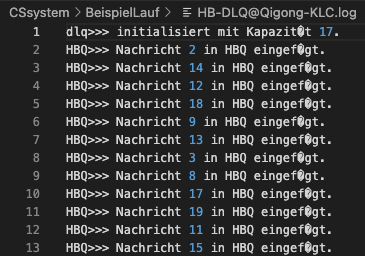
\includegraphics[scale=0.6]{Bilder/HBQFilesEntry.png}
\caption{\label{fig:HBQFilesEntry2} Nachrichtendienst \cite{HBQlogging}} 
\end{center}
\end{figure}

//TODO: Fragestellungen
Kann der Algorithmus sortieren während er die passenden Nachrichten an die Delivery-Queue ausliefert?